\documentclass[a4paper]{article}

\usepackage{pdp}
\usepackage{booktabs}
\usepackage{float}
\usepackage{enumitem}
\usepackage{amsmath}
\usepackage{multicol}

% Code listings style
\setminted{
    fontsize=\small,
    breaklines=true,
    frame=single,
    bgcolor=gray!10
}

%------------------------------------------------------------------------------
%	REPORT INFORMATION
%------------------------------------------------------------------------------

\title{Amazones -- Python}
\subtitle{Rapport préliminaire}
\author{Messaoudi Ismail, Mohammed Amine Rabih , Mohamed Ali Chaoui, Ayoub oubakki, Mahmoud Mounouar}

%------------------------------------------------------------------------------

\begin{document}

%------------------------------------------------------------------------------
%	TITLE PAGE
%------------------------------------------------------------------------------

\maketitle
\thispagestyle{empty}

%------------------------------------------------------------------------------
%	INTRODUCTION
%------------------------------------------------------------------------------

\section*{Introduction}

Ce projet s'inscrit dans le cadre du module Projet de Programmation du Master Informatique 2025--2026. Il vise à concevoir une application logicielle permettant de jouer au jeu de plateau \textit{Amazones}, un jeu à deux joueurs, déterministe et à information parfaite.

Le jeu des Amazones combine des éléments des échecs et du Go. Malgré des règles simples, il possède une grande profondeur stratégique. Sa complexité PSPACE-complète \cite{hearn2005} en fait un support pertinent pour l'étude des algorithmes d'intelligence artificielle. Plusieurs solveurs performants \cite{song2015} ont été développés pour ce jeu, démontrant l'intérêt de la communauté scientifique.



\subsection*{Spécifications techniques}

\begin{table}[H]
\centering
\begin{tabular}{ll}
\toprule
\textbf{Élément} & \textbf{Choix} \\
\midrule
Langage & Python 3.10+ \\
Build-system & pyproject.toml + setuptools \\
Interface graphique & PyGObject (GTK 4.x) \\
Framework de tests & pytest + coverage ($\geq$ 85\%) \\
Documentation & Sphinx \\
Internationalisation & gettext (anglais par défaut, français) \\
Machine Learning & Keras \\
Style de codage & PEP8 \\
\bottomrule
\end{tabular}
\caption{Stack technique du projet}
\end{table}

%------------------------------------------------------------------------------
%	PRÉSENTATION DU JEU
%------------------------------------------------------------------------------

\section{Présentation du jeu des Amazones}

\subsection{Règles du jeu et Spécifications Algorithmiques}

Le jeu se déroule sur un plateau de taille $10 \times 10$ (configurable de $4 \times 4$ à $11 \times 11$). Chaque joueur contrôle quatre amazones (sauf pour les petits plateaux $4 \times 4$ et $5 \times 5$).

\begin{figure}[H]
\centering
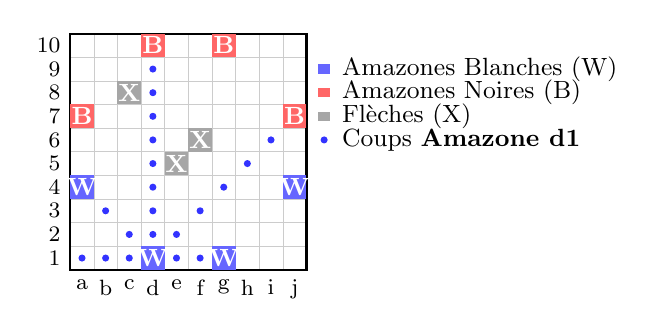
\begin{tikzpicture}[scale=0.3]
    \tikzset{
        gridstyle/.style={step=1cm, gray!40, very thin},
        borderstyle/.style={thick, black}
    }
    
    % Grille 10x10
    \draw[gridstyle] (0,0) grid (10,10);
    \draw[borderstyle] (0,0) rectangle (10,10);
    
    % Coordonnées X (a-j)
    \foreach \x/\l in {0/a,1/b,2/c,3/d,4/e,5/f,6/g,7/h,8/i,9/j} {
        \node[below, font=\footnotesize] at (\x+0.5, 0) {\l};
    }
    
    % Coordonnées Y (1-10)
    \foreach \y in {1,...,10} {
        \node[left, font=\footnotesize] at (0, \y-0.5) {\y};
    }
    
    % -- INDICATEURS DE MOUVEMENT (Points) --
    
    % 1. Pour l'Amazone Blanche en d1 (3,0) -> Bleu
    % Nord: (3,1) à (3,8) [d10(3,9) occupé]
    \foreach \y in {1,...,8} \fill[blue!80] (3.5, \y+0.5) circle (0.15);
    % Ouest: (2,0), (1,0), (0,0)
    \foreach \x in {0,1,2} \fill[blue!80] (\x+0.5, 0.5) circle (0.15);
    % Est: (4,0), (5,0) [g1(6,0) occupé]
    \foreach \x in {4,5} \fill[blue!80] (\x+0.5, 0.5) circle (0.15);
    % NW: (2,1), (1,2) [a4(0,3) occupé]
    \fill[blue!80] (2.5, 1.5) circle (0.15);
    \fill[blue!80] (1.5, 2.5) circle (0.15);
    % NE: (4,1), (5,2), (6,3), (7,4), (8,5) [j7(9,6) occupé]
    \foreach \i in {1,...,5} \fill[blue!80] (3.5+\i, 0.5+\i) circle (0.15);
    
    % 2. Pour la Flèche en f6 (5,5) -> Gris (SUPPRIMÉ pour clarté)
    % Nord: (5,6) à (5,9)
    % \foreach \y in {6,...,9} \fill[gray!80] (5.5, \y+0.5) circle (0.15);
    % Sud: (5,4) à (5,0) [f5 libre?] Wait, f5 is free. e5(4,4) is Arrow.
    % \foreach \y in {0,...,4} \fill[gray!80] (5.5, \y+0.5) circle (0.15);
    % Ouest: (4,5) à (0,5)
    % \foreach \x in {0,...,4} \fill[gray!80] (\x+0.5, 5.5) circle (0.15);
    % Est: (6,5) à (9,5)
    % \foreach \x in {6,...,9} \fill[gray!80] (\x+0.5, 5.5) circle (0.15);
    % NW: (4,6), (3,7), (2,8), (1,9)
    % \foreach \i in {1,...,4} \fill[gray!80] (5.5-\i, 5.5+\i) circle (0.15);
    % NE: (6,6), (7,7), (8,8), (9,9)
    % \foreach \i in {1,...,4} \fill[gray!80] (5.5+\i, 5.5+\i) circle (0.15);
    % SE: (6,4), (7,3), (8,2), (9,1)
    % \foreach \i in {1,...,4} \fill[gray!80] (5.5+\i, 5.5-\i) circle (0.15);
    % SW: (4,4)? Non, c'est e5(4,4) qui est une Flèche -> Bloqué.
    
    % Amazones Blanches (positions standard: a4, d1, g1, j4)
    \fill[blue!60] (0,3) rectangle (1,4);
    \fill[blue!60] (3,0) rectangle (4,1);
    \fill[blue!60] (6,0) rectangle (7,1);
    \fill[blue!60] (9,3) rectangle (10,4);
    \node[font=\small\bfseries, white] at (0.5,3.5) {W};
    \node[font=\small\bfseries, white] at (3.5,0.5) {W};
    \node[font=\small\bfseries, white] at (6.5,0.5) {W};
    \node[font=\small\bfseries, white] at (9.5,3.5) {W};
    
    % Amazones Noires (positions standard: a7, d10, g10, j7)
    \fill[red!60] (0,6) rectangle (1,7);
    \fill[red!60] (3,9) rectangle (4,10);
    \fill[red!60] (6,9) rectangle (7,10);
    \fill[red!60] (9,6) rectangle (10,7);
    \node[font=\small\bfseries, white] at (0.5,6.5) {B};
    \node[font=\small\bfseries, white] at (3.5,9.5) {B};
    \node[font=\small\bfseries, white] at (6.5,9.5) {B};
    \node[font=\small\bfseries, white] at (9.5,6.5) {B};
    
    % Flèches (3 cases bloquées: e5, f6, c8)
    \fill[gray!70] (4,4) rectangle (5,5);
    \fill[gray!70] (5,5) rectangle (6,6);
    \fill[gray!70] (2,7) rectangle (3,8);
    \node[font=\small\bfseries, white] at (4.5,4.5) {X};
    \node[font=\small\bfseries, white] at (5.5,5.5) {X};
    \node[font=\small\bfseries, white] at (2.5,7.5) {X};
    
    % Légende
    \fill[blue!60] (10.5, 8.3) rectangle (11, 8.7);
    \node[right, font=\small] at (11.1, 8.5) {Amazones Blanches (W)};
    \fill[red!60] (10.5, 7.3) rectangle (11, 7.7);
    \node[right, font=\small] at (11.1, 7.5) {Amazones Noires (B)};
    \fill[gray!70] (10.5, 6.3) rectangle (11, 6.7);
    \node[right, font=\small] at (11.1, 6.5) {Flèches (X)};
    
    \fill[blue!80] (10.75, 5.5) circle (0.15);
    \node[right, font=\small] at (11.1, 5.5) {Coups \textbf{Amazone d1}};
    
\end{tikzpicture}
\caption{Plateau de jeu $10 \times 10$ avec positions initiales et visualisation des cases accessibles (points) pour l'amazone en d1.}
\label{fig:plateau_jeu}
\end{figure}

\subsubsection{Algorithme de Déplacement}

Pour garantir une implémentation robuste, le déplacement d’une Amazone (et le tir de flèche) suit une logique vectorielle :

\begin{enumerate}
    \item L’algorithme parcourt les 8 directions cardinales et intercardinales :
    \[
    DIRS = \{(1,0), (-1,0), (0,1), (0,-1), (1,1), (-1,-1), (1,-1), (-1,1)\}
    \]
    \item Pour chaque direction $\vec{d} \in DIRS$, on progresse case par case tant que la case suivante est \textbf{VIDE} (\texttt{EMPTY}).
    \item \textbf{Condition d’arrêt} : la propagation s’arrête dès qu’un obstacle (Amazone ou Flèche) ou le bord du plateau est atteint.
\end{enumerate}

\noindent\textit{Note technique : Cette logique constitue la définition fonctionnelle. L’implémentation technique traduira ces vecteurs en masques binaires pour le module Bitboard (voir section Structures de données) afin d’optimiser les performances.}

\subsubsection{Conditions de Fin de Partie (F10)}

La partie se termine lorsqu’un joueur ne peut plus effectuer de coup légal (mouvement + tir). Ce joueur perd la partie.

\textbf{Cas particuliers :}
\begin{itemize}
    \item \textbf{Séparation du plateau} : si le plateau est divisé en zones isolées (Amazones blanches d’un côté, Noires de l’autre), le jeu \textbf{continue}.
    \item \textbf{Course de remplissage} : chaque joueur joue dans son territoire jusqu’à épuisement total des coups possibles.
    \item \textbf{Déterminisme} : le jeu des Amazones est fini et déterministe. Le nombre de cases libres diminue strictement de 1 à chaque tour (tir de flèche). Le match nul est impossible : il existe toujours un vainqueur.
\end{itemize}

\subsubsection{Gestion des Erreurs et Validité (F11)}

Le moteur de jeu doit garantir qu’aucun coup illégal n’altère l’état de la partie. Conformément à l’exigence \textbf{F11} :

\begin{itemize}
    \item Tout coup ne respectant pas l’algorithme de déplacement (traversée d’obstacle, case d’arrivée occupée) est immédiatement rejeté.
    \item Un message d’erreur explicite est retourné à l’interface (ex : \textit{"Coup invalide : Trajectoire bloquée en d4"}).
    \item Le joueur est invité à recommencer sa saisie sans pénalité.
\end{itemize}

\subsection{Placement initial des amazones (grille réglable)}

\textbf{Problème :} Comment placer les amazones sur une grille de taille variable $N \times N$ tout en garantissant la jouabilité ? Conserver quatre amazones sur de petits plateaux entraîne une saturation excessive de l’espace (densité $> 30\%$).

Nous adoptons une stratégie adaptative basée sur la réduction du nombre de pièces pour les petites grilles et une formule géométrique proportionnelle pour les tailles standards.

\begin{table}[H]
\centering
\begin{tabular}{ccl}
\toprule
\textbf{Taille ($N \times N$)} & \textbf{Nb Amazones} & \textbf{Stratégie de placement} \\
\midrule
$4 \times 4$ & 2 & Coins opposés (Densité 25\%) \\
$5 \times 5$ & 3 & Triangle (Densité 24\%) \\
$6 \times 6$ à $11 \times 11$ & 4 & Formule des Tiers (Densité 22\% à 8\%) \\
\bottomrule
\end{tabular}
\caption{Stratégies de placement adaptatives selon la taille}
\end{table}

\subsubsection{Algorithme des Tiers (pour $N \geq 6$)}

Pour placer les 4 amazones de manière équilibrée, on calcule l’indice de tiers :
\[
T = \left\lfloor \frac{N}{3} \right\rfloor
\]

Les positions du joueur \textbf{Blanc} (bas du plateau — Ligne 0) sont définies comme suit :
\begin{itemize}
    \item \textbf{Ailes :} Ligne $T$, Colonnes $0$ et $N-1$.
    \item \textbf{Centre-arrière :} Ligne $0$, Colonnes $T$ et $N-1-T$.
\end{itemize}

Le placement des Noirs est obtenu par symétrie centrale. Cette méthode garantit une ouverture équilibrée, évite le contact immédiat et favorise le contrôle des zones stratégiques.

\subsection{Notation algébrique (F20)}

Les cases sont repérées par une colonne (de \texttt{a} à \texttt{j} pour un plateau $10 \times 10$) et une ligne (de \texttt{1} à \texttt{10}).  
Les coups suivent la notation algébrique standard.

\textbf{Exemple :}  
\texttt{e2-e4/e6} signifie déplacer une amazone de \texttt{e2} vers \texttt{e4}, puis tirer une flèche sur la case \texttt{e6}.

%------------------------------------------------------------------------------
%   STRUCTURES DE DONNÉES
%------------------------------------------------------------------------------

\section{Structures de données}

\subsection{Module Bitboard}

Conformément aux exigences F26 et F27 du cahier des charges, le plateau de jeu est représenté à l'aide de \textbf{bitboards}. Cette structure de données, issue des moteurs d'échecs \cite{browne2014}, encode l'état du jeu sous forme d'entiers binaires, permettant des opérations en temps constant $O(1)$.

\subsubsection{Définition et structure}

Un \textit{bitboard} est un entier de $n^2$ bits représentant un plateau de taille $n \times n$. Chaque bit correspond à une case unique du plateau :
\begin{itemize}[noitemsep]
    \item \textbf{bit = 1} $\rightarrow$ présence de l'objet sur cette case
    \item \textbf{bit = 0} $\rightarrow$ absence de l'objet sur cette case
\end{itemize}

L'état complet du jeu est représenté par \textbf{exactement trois bitboards distincts}, chacun dédié à un type d'objet unique :

\begin{table}[H]
\centering
\begin{tabular}{lp{9cm}}
\toprule
\textbf{Bitboard} & \textbf{Contenu (exclusif)} \\
\midrule
\texttt{white\_amazons} & Positions des amazones blanches uniquement \\
\texttt{black\_amazons} & Positions des amazones noires uniquement \\
\texttt{blocked} & Positions des cases bloquées (flèches) uniquement \\
\bottomrule
\end{tabular}
\caption{Les trois bitboards représentant l'état du jeu}
\end{table}

\textbf{Règle fondamentale :} Aucun bitboard ne mélange plusieurs types d'objets. Cette séparation stricte garantit l'intégrité des opérations binaires.

\subsubsection{Indexation des cases}

Chaque case du plateau possède un index unique calculé par la formule :
\[ \texttt{index} = \texttt{ligne} \times n + \texttt{colonne} \]

où $n$ est la taille du plateau, et \texttt{ligne}, \texttt{colonne} $\in [0, n-1]$.

\begin{table}[H]
\centering
\begin{tabular}{cccc}
\toprule
\textbf{Case (affichée)} & \textbf{Coord. interne} & \textbf{Calcul ($n=10$)} & \textbf{Index} \\
\midrule
\texttt{a1} & $(0, 0)$ & $0 \times 10 + 0$ & \textbf{0} \\
\texttt{d4} & $(3, 3)$ & $3 \times 10 + 3$ & \textbf{33} \\
\texttt{j10} & $(9, 9)$ & $9 \times 10 + 9$ & \textbf{99} \\
\bottomrule
\end{tabular}
\caption{Correspondance notation algébrique $\leftrightarrow$ index bitboard (plateau $10 \times 10$)}
\end{table}

\textbf{Note :} L'affichage utilisateur (lignes 1 à 10, colonnes a-j) est une simple conversion de la représentation interne.

\subsubsection{Combinaison des bitboards}

Pour déterminer l'ensemble des cases occupées, on combine les trois bitboards par l'opération \texttt{OR} logique :
\[ \texttt{occupied} = \texttt{white\_amazons} \mid \texttt{black\_amazons} \mid \texttt{blocked} \]

Cette opération produit un nouveau bitboard où chaque bit à 1 indique une case occupée, indépendamment du type d'objet.

\begin{figure}[H]
\centering
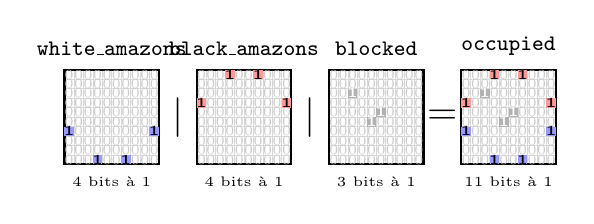
\begin{tikzpicture}[scale=0.12]
    \tikzset{
        gridstyle/.style={step=1cm, gray!30, very thin},
        borderstyle/.style={thick, black},
        bitone/.style={font=\tiny\bfseries},
        bitzero/.style={font=\tiny, gray!40}
    }

    % --- BITBOARD 1: WHITE AMAZONS (10x10) ---
    \begin{scope}
        \draw[gridstyle] (0,0) grid (10,10);
        \draw[borderstyle] (0,0) rectangle (10,10);
        \node[above, align=center] at (5,10.5) {\footnotesize \texttt{white\_amazons}};
        
        % Tous les 0 d'abord
        \foreach \x in {0,...,9} {
            \foreach \y in {0,...,9} {
                \node[bitzero] at (\x+0.5,\y+0.5) {0};
            }
        }
        
        % 4 amazones blanches (positions standard)
        \fill[blue!40] (0,3) rectangle (1,4);   % a4
        \fill[blue!40] (3,0) rectangle (4,1);   % d1
        \fill[blue!40] (6,0) rectangle (7,1);   % g1
        \fill[blue!40] (9,3) rectangle (10,4);  % j4
        \node[bitone] at (0.5,3.5) {1};
        \node[bitone] at (3.5,0.5) {1};
        \node[bitone] at (6.5,0.5) {1};
        \node[bitone] at (9.5,3.5) {1};
        
        \node[below] at (5,-0.3) {\tiny 4 bits à 1};
    \end{scope}

    \node at (12, 5) {\Large $|$};

    % --- BITBOARD 2: BLACK AMAZONS ---
    \begin{scope}[xshift=14cm]
        \draw[gridstyle] (0,0) grid (10,10);
        \draw[borderstyle] (0,0) rectangle (10,10);
        \node[above, align=center] at (5,10.5) {\footnotesize \texttt{black\_amazons}};
        
        % Tous les 0
        \foreach \x in {0,...,9} {
            \foreach \y in {0,...,9} {
                \node[bitzero] at (\x+0.5,\y+0.5) {0};
            }
        }
        
        % 4 amazones noires (positions standard)
        \fill[red!40] (0,6) rectangle (1,7);    % a7
        \fill[red!40] (3,9) rectangle (4,10);   % d10
        \fill[red!40] (6,9) rectangle (7,10);   % g10
        \fill[red!40] (9,6) rectangle (10,7);   % j7
        \node[bitone] at (0.5,6.5) {1};
        \node[bitone] at (3.5,9.5) {1};
        \node[bitone] at (6.5,9.5) {1};
        \node[bitone] at (9.5,6.5) {1};
        
        \node[below] at (5,-0.3) {\tiny 4 bits à 1};
    \end{scope}

    \node at (26, 5) {\Large $|$};

    % --- BITBOARD 3: BLOCKED ---
    \begin{scope}[xshift=28cm]
        \draw[gridstyle] (0,0) grid (10,10);
        \draw[borderstyle] (0,0) rectangle (10,10);
        \node[above, align=center] at (5,10.5) {\footnotesize \texttt{blocked}};
        
        % Tous les 0
        \foreach \x in {0,...,9} {
            \foreach \y in {0,...,9} {
                \node[bitzero] at (\x+0.5,\y+0.5) {0};
            }
        }
        
        % 3 flèches
        \fill[gray!60] (4,4) rectangle (5,5);
        \fill[gray!60] (5,5) rectangle (6,6);
        \fill[gray!60] (2,7) rectangle (3,8);
        \node[bitone, white] at (4.5,4.5) {1};
        \node[bitone, white] at (5.5,5.5) {1};
        \node[bitone, white] at (2.5,7.5) {1};
        
        \node[below] at (5,-0.3) {\tiny 3 bits à 1};
    \end{scope}

    \node at (40, 5) {\Large $=$};

    % --- OCCUPIED (résultat OR) ---
    \begin{scope}[xshift=42cm]
        \draw[gridstyle] (0,0) grid (10,10);
        \draw[borderstyle] (0,0) rectangle (10,10);
        \node[above, align=center] at (5,10.5) {\footnotesize \texttt{occupied}};
        
        % Tous les 0
        \foreach \x in {0,...,9} {
            \foreach \y in {0,...,9} {
                \node[bitzero] at (\x+0.5,\y+0.5) {0};
            }
        }
        
        % Tous les 1 combinés
        \fill[blue!40] (0,3) rectangle (1,4);
        \fill[blue!40] (3,0) rectangle (4,1);
        \fill[blue!40] (6,0) rectangle (7,1);
        \fill[blue!40] (9,3) rectangle (10,4);
        \fill[red!40] (0,6) rectangle (1,7);
        \fill[red!40] (3,9) rectangle (4,10);
        \fill[red!40] (6,9) rectangle (7,10);
        \fill[red!40] (9,6) rectangle (10,7);
        \fill[gray!60] (4,4) rectangle (5,5);
        \fill[gray!60] (5,5) rectangle (6,6);
        \fill[gray!60] (2,7) rectangle (3,8);
        
        \node[bitone] at (0.5,3.5) {1};
        \node[bitone] at (3.5,0.5) {1};
        \node[bitone] at (6.5,0.5) {1};
        \node[bitone] at (9.5,3.5) {1};
        \node[bitone] at (0.5,6.5) {1};
        \node[bitone] at (3.5,9.5) {1};
        \node[bitone] at (6.5,9.5) {1};
        \node[bitone] at (9.5,6.5) {1};
        \node[bitone, white] at (4.5,4.5) {1};
        \node[bitone, white] at (5.5,5.5) {1};
        \node[bitone, white] at (2.5,7.5) {1};
        
        \node[below] at (5,-0.3) {\tiny 11 bits à 1};
    \end{scope}

\end{tikzpicture}
\caption{Représentation binaire sur plateau $10 \times 10$ : 0 (case vide), 1 (case occupée). L'opération OR combine les bits.}
\label{fig:three_bitboards}
\end{figure}

\subsubsection{Visualisation des opérations critiques}

Les figures suivantes détaillent la mécanique interne des opérations de validation et de déplacement.

\paragraph{Validation d'un coup (Lecture)}

Pour vérifier si un coup est valide (ex: déplacement \texttt{d1} vers \texttt{d4}), on utilise des masques binaires et l'opérateur \texttt{AND}. L'algorithme :
\begin{enumerate}
    \item Agrège tous les obstacles (reines + flèches) via \texttt{OR}.
    \item Applique un masque du chemin voulu.
    \item Vérifie l'intersection via \texttt{AND}. Une valeur non nulle indique une collision.
\end{enumerate}

\begin{figure}[H]
\centering

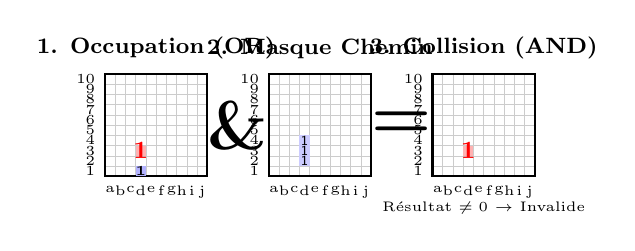
\begin{tikzpicture}[scale=0.13]
    \tikzset{
        gridstyle/.style={step=1cm, gray!40, very thin},
        borderstyle/.style={thick, black},
        bittext/.style={font=\tiny\sffamily}
    }

    % --- 1. OCCUPANCY ---
    \begin{scope}[local bounding box=Occupancy]
        \draw[gridstyle] (0,0) grid (10,10);
        \draw[borderstyle] (0,0) rectangle (10,10);
        
        \node[above, align=center] at (5,10.5) {\footnotesize \textbf{1. Occupation (OR)}};
        
        % Coordonnées
        \foreach \x/\l in {0/a,1/b,2/c,3/d,4/e,5/f,6/g,7/h,8/i,9/j} {
            \node[below, font=\tiny] at (\x+0.5, 0) {\l};
        }
        \foreach \y in {1,...,10} {
            \node[left, font=\tiny] at (0, \y-0.5) {\y};
        }
        
        % Obstacle en d3 (colonne 3, ligne 2)
        \fill[red!30] (3,2) rectangle (4,3);
        \node[red, font=\small\bfseries] at (3.5,2.5) {1};
        
        % Départ (d1)
        \fill[blue!30] (3,0) rectangle (4,1);
        \node[font=\tiny\bfseries] at (3.5,0.5) {1};
    \end{scope}

    \node at (13, 5) {\Huge \textbf{\&}};

    % --- 2. MASQUE ---
    \begin{scope}[xshift=16cm, local bounding box=Mask]
        \draw[gridstyle] (0,0) grid (10,10);
        \draw[borderstyle] (0,0) rectangle (10,10);
        
        \node[above, align=center] at (5,10.5) {\footnotesize \textbf{2. Masque Chemin}};
        
        % Coordonnées
        \foreach \x/\l in {0/a,1/b,2/c,3/d,4/e,5/f,6/g,7/h,8/i,9/j} {
            \node[below, font=\tiny] at (\x+0.5, 0) {\l};
        }
        \foreach \y in {1,...,10} {
            \node[left, font=\tiny] at (0, \y-0.5) {\y};
        }
        
        % Le chemin (d2, d3, d4)
        \fill[blue!20] (3,1) rectangle (4,2);
        \fill[blue!20] (3,2) rectangle (4,3);
        \fill[blue!20] (3,3) rectangle (4,4);
        
        \node[bittext] at (3.5,1.5) {1};
        \node[bittext] at (3.5,2.5) {1};
        \node[bittext] at (3.5,3.5) {1};
    \end{scope}

    \node at (29, 5) {\Huge \textbf{=}};

    % --- 3. RESULTAT ---
    \begin{scope}[xshift=32cm, local bounding box=Result]
        \draw[gridstyle] (0,0) grid (10,10);
        \draw[borderstyle] (0,0) rectangle (10,10);
        
        \node[above, align=center] at (5,10.5) {\footnotesize \textbf{3. Collision (AND)}};
        
        % Coordonnées
        \foreach \x/\l in {0/a,1/b,2/c,3/d,4/e,5/f,6/g,7/h,8/i,9/j} {
            \node[below, font=\tiny] at (\x+0.5, 0) {\l};
        }
        \foreach \y in {1,...,10} {
            \node[left, font=\tiny] at (0, \y-0.5) {\y};
        }
        
        % La collision (rouge vif pour bien contraster)
        \fill[red!30] (3,2) rectangle (4,3); 
        \node[red, font=\small\bfseries] at (3.5,2.5) {1};
        
        \node[below, align=center] at (5,-1.5) {\tiny Résultat $\neq 0$ $\rightarrow$ Invalide};
    \end{scope}

\end{tikzpicture}
\caption{Validation d'un coup : L'opération \texttt{AND} détecte la collision sur un plateau $10 \times 10$.}
\label{fig:bitboard_collision}
\end{figure}

\vspace{0.3cm}

\paragraph{Application d'un coup (Écriture)}

Le déplacement ne se fait pas par copie, mais par manipulation directe via \texttt{XOR} et \texttt{OR}.
Pour déplacer une amazone de \texttt{d1} (index 3) vers \texttt{d4} (index 33) :

\begin{figure}[H]
\centering
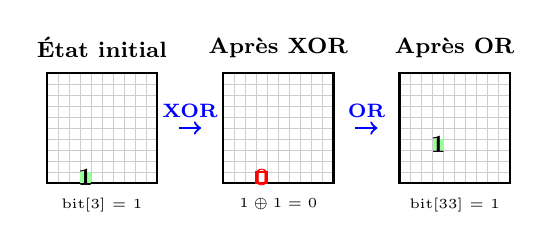
\begin{tikzpicture}[scale=0.14]
    \tikzset{
        gridstyle/.style={step=1cm, gray!40, very thin},
        borderstyle/.style={thick, black}
    }

    % --- 1. ETAT INITIAL ---
    \begin{scope}
        \draw[gridstyle] (0,0) grid (10,10);
        \draw[borderstyle] (0,0) rectangle (10,10);
        \node[above] at (5,10.5) {\footnotesize \textbf{État initial}};
        
        \fill[green!40] (3,0) rectangle (4,1);
        \node[font=\small\bfseries] at (3.5,0.5) {1};
        
        \node[below] at (5,-0.5) {\tiny bit[3] = 1};
    \end{scope}

    \draw[->, thick, blue] (12,5) -- (14,5) node[midway, above, font=\scriptsize] {\textbf{XOR}};

    % --- 2. APRES XOR ---
    \begin{scope}[xshift=16cm]
        \draw[gridstyle] (0,0) grid (10,10);
        \draw[borderstyle] (0,0) rectangle (10,10);
        \node[above] at (5,10.5) {\footnotesize \textbf{Après XOR}};
        
        \draw[red, thick] (3,0) rectangle (4,1); 
        \node[red, font=\small\bfseries] at (3.5,0.5) {0};
        
        \node[below] at (5,-0.5) {\tiny $1 \oplus 1 = 0$};
    \end{scope}

    \draw[->, thick, blue] (28,5) -- (30,5) node[midway, above, font=\scriptsize] {\textbf{OR}};

    % --- 3. APRES OR ---
    \begin{scope}[xshift=32cm]
        \draw[gridstyle] (0,0) grid (10,10);
        \draw[borderstyle] (0,0) rectangle (10,10);
        \node[above] at (5,10.5) {\footnotesize \textbf{Après OR}};
        
        \fill[green!40] (3,3) rectangle (4,4);
        \node[font=\small\bfseries] at (3.5,3.5) {1};
        
        \node[below] at (5,-0.5) {\tiny bit[33] = 1};
    \end{scope}

\end{tikzpicture}
\caption{Déplacement d'une amazone : XOR retire, OR place (plateau $10 \times 10$).}
\label{fig:bitboard_move}
\end{figure}

\subsubsection{Algorithmes de manipulation (F27)}

\noindent\textit{Note : Dans cette section, les exemples et formules utilisent un plateau de taille $10 \times 10$ (configuration standard). L'implémentation finale supportera toutes les tailles de $4 \times 4$ à $11 \times 11$ en paramétrant $n$ dans les calculs d'index et les masques de bords.}

Le cahier des charges impose cinq opérations. Voici leur conception détaillée.

\paragraph{Opération 1 : Vérifier si un coup est valide}

\textbf{Algorithme :}
\begin{enumerate}[noitemsep]
    \item Vérifier présence amazone en \texttt{from} : $(\texttt{my\_amazons} \land (1 \ll \texttt{from})) \neq 0$
    \item Vérifier alignement ligne/colonne/diagonale
    \item Vérifier chemin libre : combiner obstacles $\texttt{occupé} = \texttt{white} \mid \texttt{black} \mid \texttt{blocked}$ puis tester intersection
    \item Vérifier flèche depuis \texttt{to} (\texttt{arrow} peut = \texttt{from})
\end{enumerate}

\paragraph{Opération 2 : Calculer les coups possibles}

\textbf{Entrée :} Couleur du joueur.

\textbf{Sortie :} Liste de tous les coups légaux (triplets \texttt{from}, \texttt{to}, \texttt{arrow}).

\textbf{1. Arithmétique des index :}
Sur un bitboard 1D de largeur $L=10$, les déplacements se traduisent par des décalages d'index constants. Comme l'index est $y \times 10 + x$, monter d'une ligne ajoute 10, se déplacer latéralement change l'unité :
\begin{itemize}[noitemsep]
    \item \textbf{Vertical} : Nord ($+10$), Sud ($-10$).
    \item \textbf{Horizontal} : Est ($+1$), Ouest ($-1$).
    \item \textbf{Diagonal} : Combinaison linéaire. Ex: NE = Nord + Est = $+10 + 1 = +11$. De même : NO ($+9$), SE ($-9$), SO ($-11$).
\end{itemize}

\textbf{2. Problème du "Wrapping" (Effet Pac-Man) :}
L'indexation linéaire crée une fausse continuité entre les bords. Exemple : Index 9 (bord droit, ligne 0) $+ 1 \rightarrow$ Index 10 (bord gauche, ligne 1). Un déplacement simple vers l'Est provoquerait une téléportation de l'autre côté du plateau.

\begin{center}
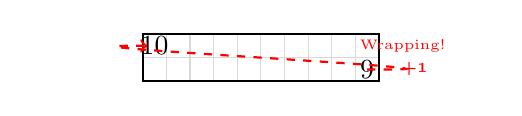
\begin{tikzpicture}[scale=0.3]
    \draw[step=1cm, gray!30] (0,0) grid (10,2);
    \draw[thick] (0,0) rectangle (10,2);
    
    % Ligne 0
    \node[anchor=center] at (9.5, 0.5) {9};
    \node[anchor=center] at (0.5, 1.5) {10};
    
    % Flèche Pac-Man
    \draw[->, red, thick, dashed] (9.5, 0.5) -- (10.5, 0.5) 
        node[right, font=\tiny] {\textbf{+1}} 
        to[out=0, in=180] (-0.5, 1.5) -- (0.2, 1.5);
        
    \node[red, font=\tiny] at (11, 1.5) {Wrapping!};
\end{tikzpicture}
\end{center}

\textbf{3. Solution par Masques de Bords :}
Le traitement des limites diffère selon l'axe :
\begin{enumerate}
    \item \textbf{Axe Horizontal (Masques)} : Pour éviter le "Wrapping", nous utilisons des masques identifiant les colonnes critiques.
    \begin{itemize}[noitemsep]
        \item \texttt{MASK\_COL\_A} : Bits à 1 sur la colonne $a$ (index 0, 10, ..., 90).
        \item \texttt{MASK\_COL\_J} : Bits à 1 sur la colonne $j$ (index 9, 19, ..., 99).
    \end{itemize}
    \item \textbf{Axe Vertical (Limites)} : Pas besoin de masque complexe. Si l'index calculé est $< 0$ ou $\ge 100$, on sort simplement du tableau (débordement haut/bas).
\end{enumerate}

\textbf{Algorithme de propagation :}
Pour chaque amazone à la position $P$ et pour chaque direction $D$ (offset) :
\begin{enumerate}
    \item Initialiser $cur = P$.
    \item Tant que la propagation est valide :
    \begin{itemize}
        \item \textbf{Vérification Anti-Wrap (Horizontal)} :
        \begin{itemize}
            \item Pour les directions ayant une composante Est (ex: $+1, -9, +11$) : si $cur \in \texttt{MASK\_COL\_J}$, alors \textbf{STOP}.
            \item Pour les directions ayant une composante Ouest (ex: $-1, +9, -11$) : si $cur \in \texttt{MASK\_COL\_A}$, alors \textbf{STOP}.
        \end{itemize}
        \item Calculer $next = cur + D$.
        \item \textbf{Vérification Verticale (Limites)} : Si $next < 0$ ou $next \ge 100$ : \textbf{STOP}.
        \item \textbf{Collision} : Si la case $next$ est occupée (test bit à 1) : \textbf{STOP}.
        \item Sinon, ajouter $next$ aux coups valides et avancer ($cur = next$).
    \end{itemize}
    \item Pour chaque destination $to$ validée, relancer cet algorithme depuis $to$ pour trouver les tirs de flèche $arrow$ (en considérant $from$ comme vide).
\end{enumerate}

\paragraph{Opération 3 : Appliquer un coup}

\textbf{Entrée :} Un coup (\texttt{from}, \texttt{to}, \texttt{arrow}).

\textbf{Effet :} Modifie l'état du plateau (voir Figure \ref{fig:bitboard_move}).

\textbf{Algorithme (Ordre strict requis) :}
\begin{enumerate}
    \item \textbf{1. Libérer la case de départ} (XOR) :
    Cette étape doit être réalisée \textbf{avant} de tirer la flèche, car la flèche peut légalement atterrir sur la case \texttt{from} qui vient d'être libérée.
    \begin{center}
    $\texttt{amazons} = \texttt{amazons} \oplus (1 \ll \texttt{from})$
    \end{center}
    
    \item \textbf{2. Occuper la case d'arrivée} (OR) :
    \begin{center}
    $\texttt{amazons} = \texttt{amazons} \mid (1 \ll \texttt{to})$
    \end{center}
    
    \item \textbf{3. Tirer la flèche} (OR) :
    La case \texttt{arrow} est marquée comme bloquée. Si \texttt{arrow} == \texttt{from}, cela fonctionne correctement car l'étape 1 a déjà libéré la place.
    \begin{center}
    $\texttt{blocked} = \texttt{blocked} \mid (1 \ll \texttt{arrow})$
    \end{center}
\end{enumerate}

\paragraph{Opération 4 : Calculer les scores}

Score = $M_{\text{joueur}} - M_{\text{adversaire}}$ où $M$ = nombre de coups possibles.

\paragraph{Opération 5 : Fin de partie}

Le joueur a perdu si aucun coup n'est possible (Opération 2 retourne liste vide).

\subsubsection{Résumé des opérations bit à bit}

\begin{table}[H]
\centering
\begin{tabular}{lll}
\toprule
\textbf{Opération} & \textbf{Notation} & \textbf{Utilisation} \\
\midrule
Shift gauche & $1 \ll n$ & Créer un masque pour la position $n$ \\
OR & $a \mid b$ & Placer une pièce ou bloquer une case \\
XOR & $a \oplus b$ & Retirer une pièce (inverser un bit) \\
AND & $a \land b$ & Tester si une case est occupée \\
\bottomrule
\end{tabular}
\caption{Récapitulatif des opérations bit à bit}
\end{table}


\subsection{Architecture logicielle}

L'architecture du projet suit le pattern MVC (Modèle-Vue-Contrôleur). La figure 1 présente le diagramme de classes.

\begin{figure}[H]
  \centering
  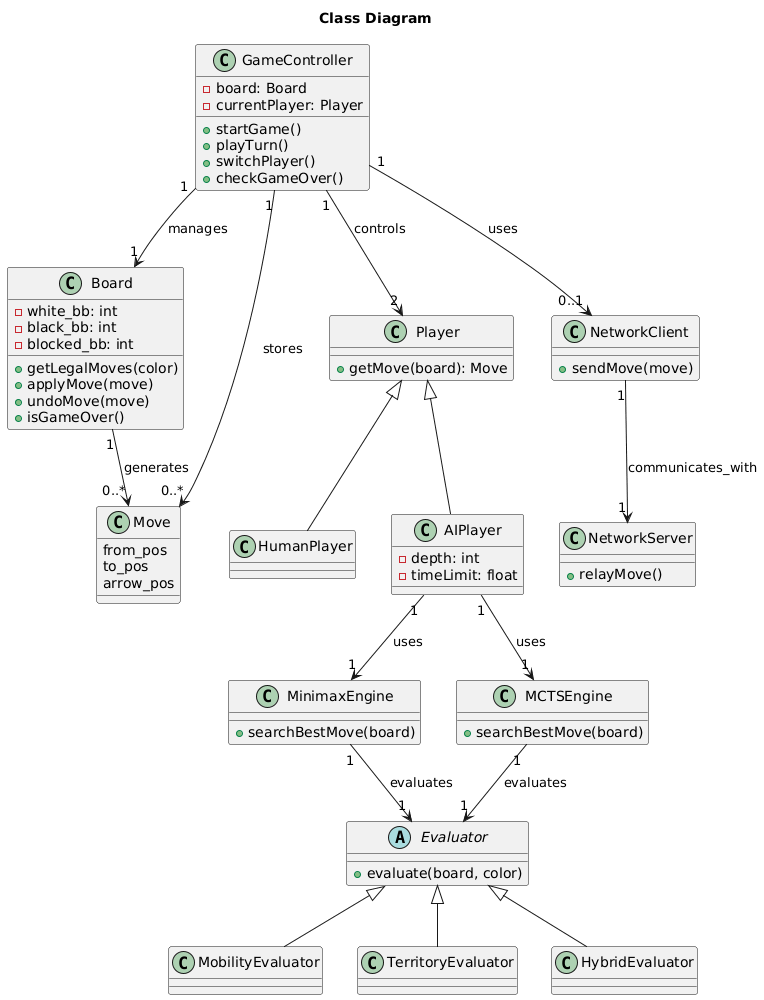
\includegraphics[width=0.65\textwidth]{diagramme-de-classe.png}
  \caption{Diagramme de classes UML \cite{plantuml}}\label{fig:classes}
\end{figure}

\begin{figure}[H]
  \centering

  \begin{minipage}{0.48\textwidth}
    \centering
    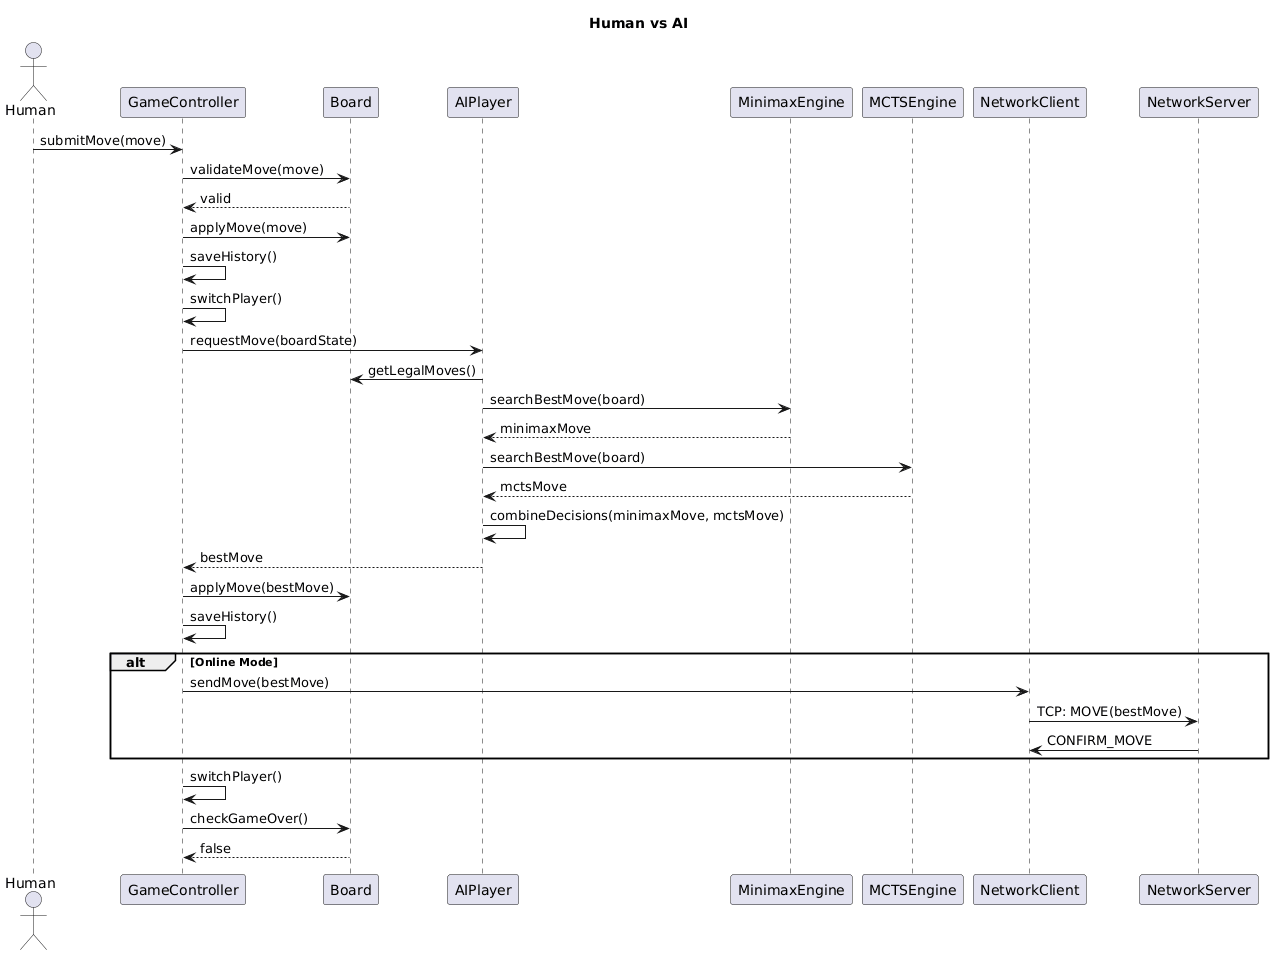
\includegraphics[width=\textwidth]{diag-seq-ai.png}
    \caption{Humain vs AI Player}
    \label{fig:sequence-ai}
  \end{minipage}
  \hfill
  \begin{minipage}{0.48\textwidth}
    \centering
    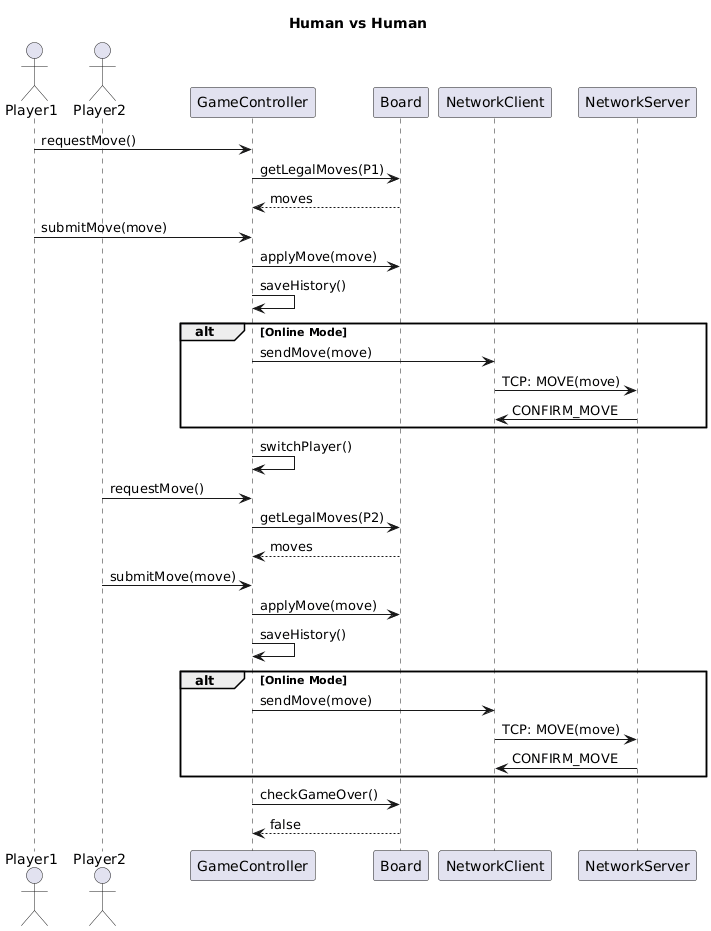
\includegraphics[width=\textwidth]{diag-seq-hum.png}
    \caption{Humain vs Humain}
    \label{fig:sequence-hum}
  \end{minipage}

\end{figure}


%------------------------------------------------------------------------------
%	INTELLIGENCE ARTIFICIELLE
%------------------------------------------------------------------------------

\section{Intelligence artificielle (IA hybride)}

Le joueur artificiel repose sur une chaîne de décision commune :

\begin{itemize}
  \item \textbf{Génération des coups légaux} : \texttt{Board.getLegalMoves(color)} produit une liste de coups \texttt{Move(from,to,arrow)}.
  \item \textbf{Recherche} : l'IA utilise deux moteurs complémentaires : \textbf{Minimax avec élagage $\alpha\beta$} et \textbf{Monte Carlo Tree Search (MCTS)}.
  \item \textbf{Évaluation} : chaque position est notée via \texttt{Evaluator.evaluate(board,color)} (mobilité, territoire ou hybride).
  \item \textbf{Fusion} : l'\texttt{AIPlayer} combine les propositions de Minimax et MCTS pour produire un \texttt{bestMove}.
\end{itemize}

\textbf{Pipeline global :}
\[
Board \rightarrow getLegalMoves \rightarrow (Minimax + MCTS) \rightarrow Evaluator \rightarrow bestMove
\]

\subsection{Minimax avec élagage $\alpha\beta$}

Minimax modélise la partie comme un arbre alternant :
\textbf{MAX} (notre tour, maximiser le score) et \textbf{MIN} (tour adverse, minimiser le score).

La recherche est limitée par une profondeur ou un budget temps.  
Si \texttt{depth = 0} ou fin de partie, on renvoie :
\[
score = evaluate(board, color)
\]

Pour explorer l’arbre, l’algorithme applique un coup avec \texttt{applyMove(move)} puis revient en arrière avec \texttt{undoMove(move)}.

L’élagage $\alpha\beta$ évite d’explorer des branches inutiles lorsque :
\[
\alpha \geq \beta
\]

\subsection{Fonctions d’évaluation}

Trois heuristiques sont implémentées via héritage de \texttt{Evaluator} :

\textbf{Mobilité :}
\[
score_{mob}(s) = |Moves(s,joueur)| - |Moves(s,adversaire)|
\]

\textbf{Territoire :}
\[
score_{terr}(s) = \#cases_{nous} - \#cases_{lui}
\]

\textbf{Hybride :}
\[
score_{hyb}(s) = \lambda \cdot score_{mob}(s) + (1-\lambda)\cdot score_{terr}(s)
\]
avec $\lambda \in [0,1]$.

\subsection{Monte Carlo Tree Search (MCTS)}

MCTS \cite{browne2012mcts} explore l’arbre par simulations successives :

\begin{itemize}
  \item Sélection (UCT)
  \item Expansion
  \item Simulation (rollout)
  \item Rétropropagation
\end{itemize}

Le critère UCT \cite{kocsis2006uct} équilibre exploration et exploitation :
\[
UCT_i = \frac{w_i}{n_i} + C \sqrt{\frac{\ln N}{n_i}}
\]

Le coup final correspond au nœud racine le plus robuste (meilleure moyenne ou plus visité).


%------------------------------------------------------------------------------
%	JEU EN RÉSEAU
%------------------------------------------------------------------------------

\section{Jeu en réseau}

\textbf{Point critique identifié :}  
La gestion du réseau constitue une partie technique sensible du projet, susceptible de bloquer son avancement si elle n’est pas anticipée correctement. Pour cette raison, une étude des différentes bibliothèques réseau disponibles en Python a été réalisée dès les premières phases de conception.

\subsection{Bibliothèques Python pour le réseau}

\begin{table}[H]
\centering
\begin{tabular}{lll}
\toprule
\textbf{Bibliothèque} & \textbf{Usage} & \textbf{Avantage} \\
\midrule
\texttt{socket} & Connexions TCP/UDP & Standard, bas niveau \\
\texttt{asyncio} & Entrées/Sorties asynchrones & Gestion multi-clients sans threads \\
\bottomrule
\end{tabular}
\caption{Bibliothèques réseau Python étudiées}
\end{table}

\textbf{Choix retenu :}  
L’architecture réseau repose sur l’utilisation conjointe des bibliothèques \texttt{socket} \cite{pythonsocket} et \texttt{asyncio} afin d’assurer une gestion asynchrone et efficace des connexions.

\textbf{Justification :}
\begin{itemize}
    \item Gestion efficace de plusieurs clients simultanément
    \item Absence de surcharge liée au multi-threading (verrou global d’interpréteur Python – GIL)
    \item Compatibilité avec la structure des données du jeu (bitboards facilement sérialisables)
\end{itemize}

\subsection{Architecture client--serveur}

\begin{figure}[H]
  \centering
  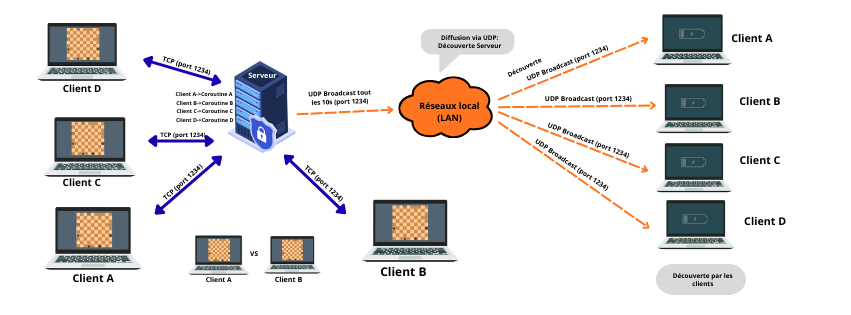
\includegraphics[width=0.95\textwidth]{shema_reseaux.png}
  \caption{Architecture réseau client--serveur du jeu}
  \label{fig:architecture_reseau}
\end{figure}

Cette architecture repose sur une séparation claire entre la phase de découverte du serveur via UDP et la phase de jeu reposant sur des connexions TCP persistantes.

\begin{itemize}
    \item Découverte automatique du serveur sur le réseau local via des messages UDP en broadcast (port 12346)
    \item Connexion des clients au serveur par TCP (port 12345 par défaut)
    \item Gestion simultanée de plusieurs clients et parties grâce à une boucle événementielle \texttt{asyncio}
    \item Système d’invitations entre joueurs avec gestion des délais d’expiration
\end{itemize}



%------------------------------------------------------------------------------
%	BESOINS FONCTIONNELS
%------------------------------------------------------------------------------

\section{Besoins fonctionnels}

Cette section liste l'ensemble des exigences fonctionnelles du cahier des charges.

\begin{table}[H]
\centering
\small
\begin{tabular}{clp{8.5cm}}
\toprule
\textbf{ID} & \textbf{Catégorie} & \textbf{Description synthétique} \\
\midrule

F1--F3 & Lancement & Options CLI, config utilisateur, internationalisation \\

F4--F9 & Modes de jeu & CLI, Blitz, Contest, GUI, IA, taille variable \\

F10--F14 & Gestion du jeu & Validation, gestion erreurs, Undo/Redo \\

F15--F20 & Interface CLI & Shell interactif, historique, notation algébrique \\

F21--F25 & Sauvegarde & Format ASCII, paramètres, état et historique \\

F26--F27 & Structures & Bitboards + algorithmes cœur du moteur \\

F28--F30 & Interface GUI & Menus, raccourcis, Drag'n'Drop \\

F31--F37 & Intelligence artificielle & Minimax, MCTS, évaluation, ML \\

F38--F40 & Réseau & Découverte UDP, TCP multi-clients, invitations \\

\bottomrule
\end{tabular}
\caption{Synthèse des besoins fonctionnels (F1--F40)}
\end{table}


%------------------------------------------------------------------------------
%	BESOINS NON FONCTIONNELS
%------------------------------------------------------------------------------

\section{Besoins non fonctionnels}


\begin{table}[H]
\centering
\begin{tabular}{lp{10cm}}
\toprule
\textbf{Exigence} & \textbf{Description} \\
\midrule
Performance & L'IA doit répondre en moins de 5 secondes par défaut \\
Portabilité & Fonctionne sur GNU/Linux (cible principale) \\
Maintenabilité & Code modulaire, couverture tests $\geq$ 85\% \\
Robustesse & Aucun crash, messages d'erreur explicites \\
Internationalisation & Support anglais (défaut) et français \\
\bottomrule
\end{tabular}
\caption{Exigences non fonctionnelles}
\end{table}

%------------------------------------------------------------------------------
%	CONCLUSION
%------------------------------------------------------------------------------

\section*{Conclusion}

Ce rapport préliminaire présente une analyse approfondie des choix techniques et méthodologiques pour le développement du jeu des Amazones. Plusieurs aspects clés ont été identifiés et traités :

\textbf{Architecture et structures de données :} L'utilisation des bitboards comme structure centrale offre des performances optimales en temps constant $O(1)$ pour toutes les opérations critiques (validation, génération de coups, application). Cette approche, inspirée des moteurs d'échecs professionnels, permet une réduction mémoire de 90\% tout en garantissant l'efficacité du moteur.

\textbf{Intelligence artificielle :} L'implémentation hybride combinant Minimax avec élagage $\alpha\beta$ et Monte Carlo Tree Search (MCTS) permet d'exploiter les forces complémentaires de ces deux approches. Le système d'évaluation heuristique (mobilité, territoire) fournit une base solide pour l'analyse stratégique.

\textbf{Architecture logicielle :} Le pattern MVC assure une séparation claire des responsabilités, facilitant la maintenance et l'évolution du code. L'architecture réseau basée sur \texttt{socket} et \texttt{asyncio} permet une gestion asynchrone efficace pour le mode multi-joueurs.

\textbf{Qualité et robustesse :} Les exigences de couverture de tests ($\geq$ 85\%), la documentation exhaustive via Sphinx, et la gestion rigoureuse des erreurs garantissent un logiciel fiable et maintenable.

Les prochaines étapes consistent à implémenter le module bitboard complet et la logique de jeu de base lors du Sprint 0, avant de passer au développement des fonctionnalités avancées (IA, réseau, interface graphique GTK4).

%------------------------------------------------------------------------------
%	BIBLIOGRAPHY
%------------------------------------------------------------------------------

\bibliographystyle{plain}
\bibliography{bibliography}

\end{document}
